
In the without front-end scenario, the processors solely start to process as soon as each processor receives its entire load assignment\cite{gamboa2011simple}.  

This subsection concerns the processors without front-end.  Because of without front-end, the processors simultaneously receive the data and solely start to process it as soon as each processor receives its entire load assignment.  \\
We consider the timing diagram for \Fig{2t2}, \Fig{2t3}, \Fig{2t10} and so on.   In addition, we also give the new closed-form matrix equations for the previous user cases.  \\
The rule also plays a dominate role in establish the mathematics model.  \\
\subsection{Data Injection on The Corner Processor}
\subsubsection{2*2 Regular Network}
The timing diagram of \Fig{2t2} is shown:

\begin{figure}[!ht]
\centering
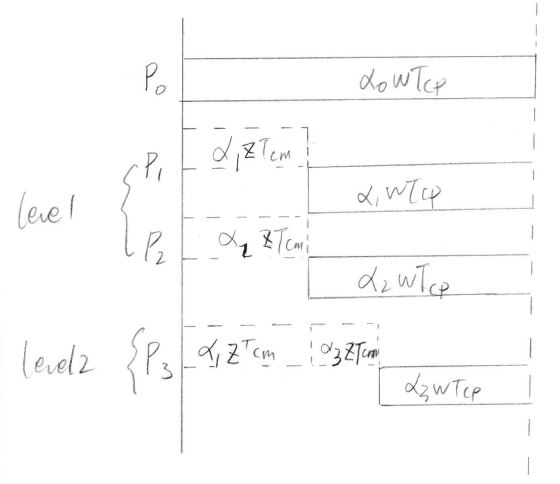
\includegraphics[width=0.5\columnwidth]{figure/2t2d_no.JPG}
\caption{The timing diagram for 2*2 regular network without front-end.  }
\label{fig:2t2d_no}
\end{figure}
\newpage 

$P_{0}$ starts to process the assigned workload and it starts to transfer the $\alpha_{1}$, $\alpha_{2}$  and $\alpha_{3}$ fraction workload after it totally receive its $\alpha_{0}$ task.  That is,  $P_{1}$ and $P_{2}$ are idle until the $L$ finish its data injection to $P_{0}.  $The similar situation happens to $P_{1}$ and $P_{2}$ and they both start to transmit the $\alpha_{3}$ after they totally receive the appropriate workload.  In other words, $P_{3}$ has to wait until the previous two layer processors obtain their own data. 

The corresponding group of equations are as follows:

\begin{empheq}[left=\empheqlbrace]
{align}
\alpha_{0} \omega T_{cp} = T_{f, m}\\
\alpha_{1}zT_{cm} + \alpha_{1} \omega T_{cp} = T_{f, m}\\
\alpha_{2}zT_{cm} + \alpha_{2} \omega T_{cp} = T_{f, m}\\
(\alpha_{1} + \alpha_{3})zT_{cm} + \alpha_{3}\omega T_{cp} = T_{f, m}\\
\sigma = \frac{zT_{cm}}{\omega T_{cp}}\\
\alpha_{0} + \alpha_{1} +\alpha_{2} + \alpha_{3} = 1\\
0 < \sigma < 1 \\
0 < \alpha_{0} \leq 1\\
0 \leq \alpha_{1},  \alpha_{2},  \alpha_{3}  < 1
\end{empheq}
\\
The matrix closed-from is presented as:
\begin{equation}
{
\left[ \begin{array}{ccc}
1 & 2 & 1\\
1 & -(\sigma + 1) & 0\\
1 & -\sigma & -(\sigma + 1)
\end{array} 
\right ]} \times \left[ \begin{array}{c}
\alpha_{0} \\
\alpha_{1} \\
\alpha_{3} 
\end{array} 
\right ] = \left[ \begin{array}{c}
1 \\
0 \\
0 
\end{array} 
\right ]
\end{equation}
\\
The explicit solution is:
\begin{empheq}[left=\empheqlbrace]
{align}
\alpha_{0} = (\frac{\sigma + 1}{\sigma + 2})^{2}\\
\alpha_{1} = \frac{\sigma + 1}{(\sigma + 2)^{2}}\\
\alpha_{3} = \frac{1}{(\sigma + 2)^{2}}
\end{empheq}
\\
The simulation result for \Fig{2t2} is provided in \Fig{2t2_no_fraction}:
\begin{figure}[!ht]
\centering
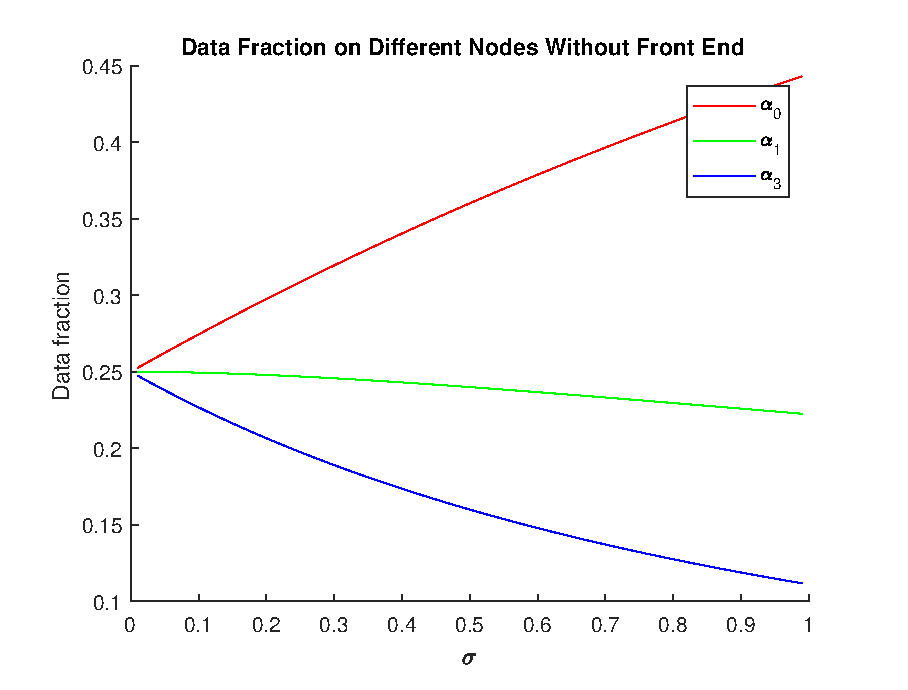
\includegraphics[width=1\columnwidth]{figure/2t2_no_fraction.eps}
\caption{The data fraction deployed based on the radius value }
\label{fig:2t2_no_fraction}
\end{figure}
\newpage

\Fig{2t2_no_fraction} explains that as the value $\sigma$ grows up,  as the fraction assigned to $P_{0}$ increases, the fractions distributed to $level_{1}$ and $level_{2}$ reduces.  In other words, if the communication capability decreases, there are more data processed locally, which is reasonable.  If the ability of the link degrades, asymptotically equaling to the processor computation capacity, there is solely $11\%$ data is deployed to the $level_{2}$.  In addition, if the $\sigma > 1$,  it means that the transmitting power is less than the processor's processing ability.  In this scenario, keeping the data locally is more economical than transmitting it.  
\newpage

\subsubsection*{2*3 Regular Network}

$P_{0}$ starts to process the assigned workload and it starts to transfer the $\alpha_{1}$, $\alpha_{2}$, $\alpha_{3}$, $\alpha_{4}$, $\alpha_{5}$ fraction workload after it totally receive its $\alpha_{0}$ task.  That is,  $P_{1}$ and $P_{2}$ are idle until the $L$ finishes its data injection to $P_{0}$.  According to the $level_{1}$, the similar situation happens to $P_{1}$ and $P_{2}$ and they both start to transmit the $\alpha_{3}$ after they totally receive the appropriate workload.  In other words, $P_{3}$ has to wait until the previous three layers,  $level_{0}$,  $level_{1}$ and $level_{2}$ processors obtain their own data.  

\begin{figure}[!ht]
\centering
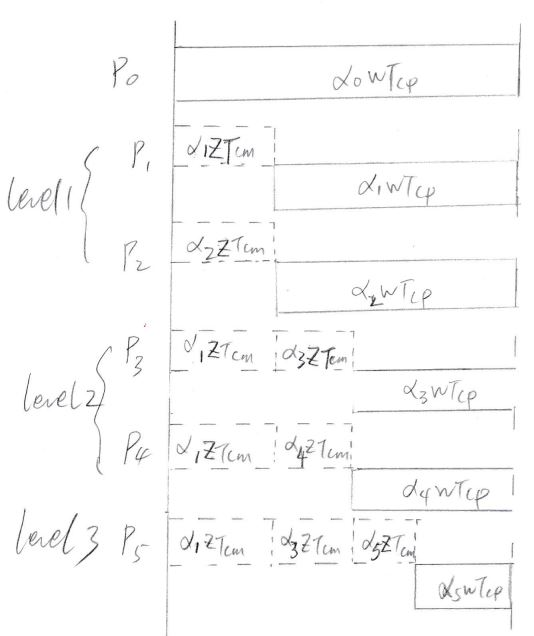
\includegraphics[width=0.65\columnwidth]{figure/2t3d_no.JPG}
\caption{The timing diagram for 2*3 regular network without front-end.  }
\label{fig:2t3d_no}
\end{figure}

In addition,  the group of equations are as follows:
\begin{empheq}[left=\empheqlbrace]
{align}
\alpha_{0} \omega T_{cp} = T_{f, m}\\
\alpha_{1}zT_{cm} + \alpha_{1} \omega T_{cp} = T_{f, m}\\
\alpha_{2}zT_{cm} + \alpha_{2} \omega T_{cp} = T_{f, m}\\
(\alpha_{1} + \alpha_{3})zT_{cm} + \alpha_{3}\omega T_{cp} = T_{f, m}\\
(\alpha_{1} + \alpha_{4})zT_{cm} + \alpha_{4}\omega T_{cp} = T_{f, m}\\
(\alpha_{1} + \alpha_{3} + \alpha_{5})zT_{cm} + \alpha_{5}\omega T_{cp} = T_{f, m}\\
\sigma = \frac{zT_{cm}}{\omega T_{cp}}\\
\alpha_{0} + \alpha_{1} +\alpha_{2} + \alpha_{3} + \alpha_{4} + \alpha_{5} = 1\\
0 < \alpha_{0} \leq 1\\
0 \leq \alpha_{1} \quad \alpha_{2} \quad \alpha_{3} \quad \alpha_{4} \quad \alpha_{5} < 1
\end{empheq}

The flow matrix is :
\begin{equation}
{
\left[ \begin{array}{cccc}
1 & 2 & 2 & 1\\
1 & -(\sigma + 1) & 0 & 0\\
1 & -\sigma & -(\sigma + 1) & 0\\
1 & -\sigma & -\sigma & -(\sigma + 1)
\end{array} 
\right ]} \times \left[ \begin{array}{c}
\alpha_{0} \\
\alpha_{1} \\
\alpha_{3} \\
\alpha_{5}
\end{array} 
\right ] = \left[ \begin{array}{c}
1 \\
0 \\
0 \\
0
\end{array} 
\right ]
\end{equation}
\\
The speedup is 
$$Speedup = \frac{T_{f, 0}}{T_{f, n}}= \frac{\omega T_{cp}}{\alpha_{0}\omega T_{cp}} = \frac{1}{\alpha_{0}}$$

The explicit solution is:
\begin{empheq}[left=\empheqlbrace]
{align}
\alpha_{0} = (\frac{\sigma + 1}{\sigma + 2})^{3}\\
\alpha_{1} = \frac{(\sigma + 1)^{2}}{(\sigma + 2)^{3}}\\
\alpha_{3} = \frac{\sigma + 1}{(\sigma + 2)^{3}}\\
\alpha_{5} = \frac{1}{(\sigma + 2)^{3}}
\end{empheq}
\\
The simulation result is:

\begin{figure}[!ht]
\centering
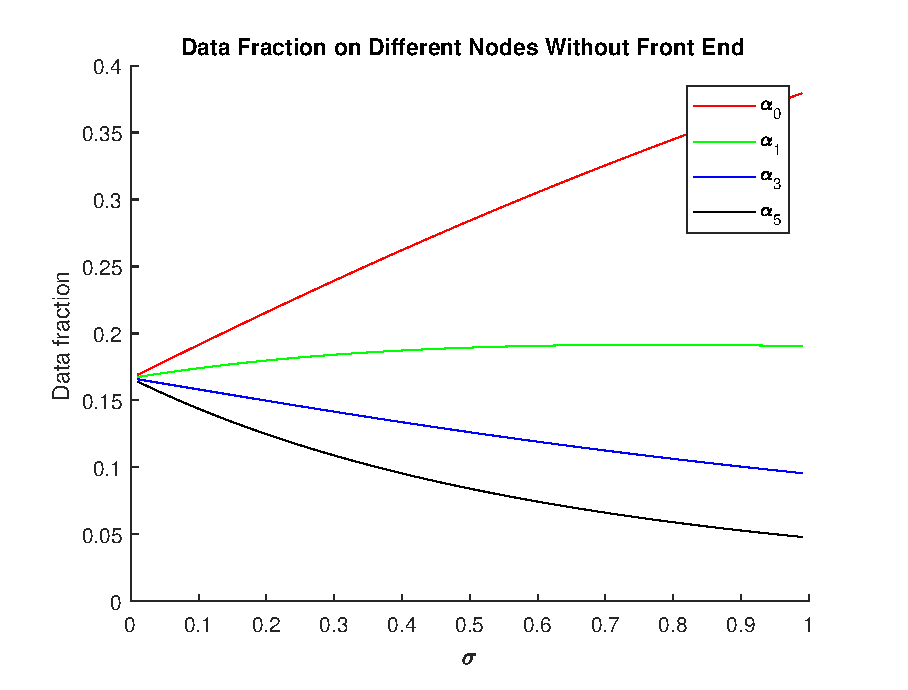
\includegraphics[width=1\columnwidth]{figure/2t3_no_fraction.eps}
\caption{The data fraction deployed based on the radius value }
\label{fig:2t3_no_fraction}
\end{figure}
\newpage

\subsubsection{2*n Regular Network}

Considering \Fig{2t10}, the equations are demonstrated as follows:

\begin{empheq}[left=\empheqlbrace]
{align}
\alpha_{0} \omega T_{cp} = T_{f, m}\\
\alpha_{1}zT_{cm} + \alpha_{1} \omega T_{cp} = T_{f, m}\\
\alpha_{2}zT_{cm} + \alpha_{2} \omega T_{cp} = T_{f, m}\\
(\alpha_{1} + \alpha_{3})zT_{cm} + \alpha_{3}\omega T_{cp} = T_{f, m}\\
(\alpha_{1} + \alpha_{4})zT_{cm} + \alpha_{4}\omega T_{cp} = T_{f, m}\\
(\alpha_{1} + \alpha_{3} + \alpha_{5})zT_{cm} + \alpha_{5}\omega T_{cp} = T_{f, m}\\
\vdots\\
(\alpha_{1} + \alpha_{3} +\cdots + \alpha_{2 \times n - 1})zT_{cm} +\alpha_{2 \times n - 1} \omega T_{cp} = T_{f, m}\\
\sigma = \frac{zT_{cm}}{\omega T_{cp}}\\
0 < \sigma < 1 \\
0 < \alpha_{0} \leq 1\\
0 \leq \quad \alpha_{1} \quad \alpha_{3} \quad  \cdots  \quad \alpha_{2 \times n - 1} < 1
\end{empheq}

Use $\sigma^{\star}$ to present $-(\sigma + 1)$ and the flow matrix form for the group of equations is :

\begin{equation}
{
\left[ \begin{array}{ccccccc}
1 & 2 & 2 & \cdots & 2 & 2 & 1\\
1 & \sigma^{\star} & 0 & \cdots& 0 & 0 & 0\\
1 & -\sigma & \sigma^{\star} & \cdots & 0 & 0 & 0 \\
1 & -\sigma & -\sigma & \sigma^{\star} & 0 & \cdots & 0 \\
1 & -\sigma & -\sigma & -\sigma & \sigma^{\star} & 0 & 0 \\
\vdots & \vdots & \vdots  &   \vdots & \ddots & \ddots\\
1 & -\sigma & -\sigma & \cdots & -\sigma & -\sigma & \sigma^{\star}
\end{array} 
\right ]} \times \left[ \begin{array}{c}
\alpha_{0} \\
\alpha_{1} \\
\alpha_{3} \\
\alpha_{5} \\
\vdots \\
\alpha_{2 \times n - 3}\\
\alpha_{2 \times n - 1}
\end{array} 
\right ] = \left[ \begin{array}{c}
1 \\
0 \\
0 \\
0 \\
\vdots \\
0
\end{array} 
\right ]
\end{equation}

According to the \textbf{\textit{Cramer's rule}},the explicit solution for the group of equations is:
\begin{empheq}[left=\empheqlbrace]
{align}
\alpha_{i} = \left |\frac{\det A^{\star}_{i}}{\det A}\right |
\end{empheq}
where $A^{\star}_{i}$ is the matrix formed by replacing the $i$-th column of A by the column vector b.
\newpage

We use  $-\sigma - 2 = \epsilon$ and $\sigma^{\star} -2 = \beta$.  After a series of column reduction and row reduction, the flow matrix changes as follows :
\begin{equation*}
     {A = \left[ \begin{array}{ccccccc}
1 & 2 & 2 & \cdots & 2 & 2 & 1\\
1 & {\sigma}^{\star} & 0 & 0 & 0 & 0 &0\\
1 & -\sigma & {\sigma}^{\star} & 0 & 0 & 0 & 0 \\
1 & -\sigma & -\sigma & {\sigma}^{\star} & 0 & 0 & 0 \\
1 & -\sigma & -\sigma & -\sigma & {\sigma}^{\star} & 0 & 0\\
1 & -\sigma & -\sigma & -\sigma & -\sigma & {\sigma}^{\star} & 0\\
1 & -\sigma & -\sigma & -\sigma & -\sigma & -\sigma & {\sigma}^{\star}\\
\end{array} 
\right ]
\xrightarrow[\text{Reduction}]{\text{Column}}\\
\left[ \begin{array}{ccccccc}
1 & 0 & 0 & \cdots & 0 & 0 & 0\\
1 & \beta & -2 & \cdots& -2 & -2 & -1\\
1 & \epsilon & \beta & \cdots & 0 & 0 & 0 \\
1 & \epsilon & \epsilon & \beta & 0 & \cdots & 0 \\
1 & \epsilon & \epsilon & \epsilon & \beta & 0 & 0 \\
\vdots & \vdots & \vdots  &   \vdots & \ddots & \ddots\\
1 & \epsilon & \epsilon & \cdots & \epsilon & \epsilon & \beta
\end{array} 
\right ]
}
\end{equation*}

\begin{equation*}
{\xrightarrow[\text{Reduction}]{\text{Row}}\\
\left[ \begin{array}{ccccccc}
1 & 0 & 0 & \cdots & 0 & 0 & 0\\
0 & \beta & -2 & \cdots& -2 & -2 & -1\\
0 & \epsilon & \beta & \cdots & 0 & 0 & 0 \\
0 & \epsilon & \epsilon & \beta & 0 & \cdots & 0 \\
0 & \epsilon & \epsilon & \epsilon & \beta & 0 & 0 \\
\vdots & \vdots & \vdots  &   \vdots & \ddots & \ddots\\
0 & \epsilon & \epsilon & \cdots & \epsilon & \epsilon & \beta
\end{array} 
\right ]
}
\end{equation*}

We define
\begin{equation*}
{C = \left[ \begin{array}{cccccc}
{\sigma}^{\star} & 0 & 0 & 0 & 0 &0\\
-\sigma & {\sigma}^{\star} & 0 & 0 & 0 & 0 \\
-\sigma & -\sigma & {\sigma}^{\star} & 0 & 0 & 0 \\
-\sigma & -\sigma & -\sigma & {\sigma}^{\star} & 0 & 0\\
-\sigma & -\sigma & -\sigma & -\sigma & {\sigma}^{\star} & 0\\
-\sigma & -\sigma & -\sigma & -\sigma & -\sigma & {\sigma}^{\star}\\
\end{array} 
\right ]
}
\end{equation*}

$0 < \sigma < 1$, then $-2 < \sigma^{\star} < -1$, which means $C$ is column linear independent, after column and row reduction. \\
Further, we define
\begin{equation*}
{\hat{C} = \left[ \begin{array}{cccccc}
\beta & -2 & \cdots& -2 & -2 & -1\\
\epsilon & \beta & \cdots & 0 & 0 & 0 \\
\epsilon & \epsilon & \beta & 0 & \cdots & 0 \\
\epsilon & \epsilon & \epsilon & \beta & 0 & 0 \\
\vdots & \vdots & \vdots  &   \vdots & \ddots & \ddots\\
\epsilon & \epsilon & \cdots & \epsilon & \epsilon & \beta
\end{array} 
\right ]
}
\end{equation*}

$C^{\star}$ is full rank.\\
So the flow matrix $A$ is full rank, that is, $\det A \neq 0$ and $\det A^{*} \neq 0$.
The speedup is  
$$Speedup = \frac{T_{f, 0}}{T_{f, n}}= \frac{\omega T_{cp}}{\alpha_{0}\omega T_{cp}} = \frac{1}{\alpha_{0}} = \frac{\det A}{\det A^{\star}} = \left |\frac{\det A}{(\sigma^{\star})^{n-1}}\right|$$
\newpage 

\subsubsection{m*n Regular Network}
Referring to \Fig{5t5}, we utilize ${\sigma}^{\star}$ to present the $-(\sigma + 1)$.  The matrix closed-form is:
\begin{equation}
{
\left[ \begin{array}{ccccccccc}
1 & 2 & 3 & 4 & 5 & 4 & 3 & 2 & 1\\
1 & {\sigma}^{\star} & 0 & 0 & 0 & 0 & 0 & 0 & 0\\
1 & -\sigma & {\sigma}^{\star} & 0 & 0 & 0 & 0& 0 & 0 \\
1 & -\sigma & -\sigma & {\sigma}^{\star} & 0 &0 & 0 & 0 & 0 \\
1 & -\sigma & -\sigma & -\sigma & {\sigma}^{\star} & 0 & 0 & 0 & 0\\
1 & -\sigma & -\sigma & -\sigma & -\sigma & {\sigma}^{\star} & 0 & 0 & 0\\
1 & -\sigma & -\sigma & -\sigma & -\sigma & -\sigma & {\sigma}^{\star} & 0 & 0\\
1 & -\sigma & -\sigma & -\sigma & -\sigma & -\sigma & -\sigma & {\sigma}^{\star} &0\\
1 & -\sigma & -\sigma & -\sigma & -\sigma & -\sigma & -\sigma & -\sigma & {\sigma}^{\star}\\
\end{array} 
\right ]} \times \left[ \begin{array}{c}
\alpha_{0} \\
\alpha_{1} \\
\alpha_{3} \\
\alpha_{6} \\
\alpha_{10} \\
\alpha_{15}\\
\alpha_{19}\\
\alpha_{22}\\
\alpha_{24}
\end{array} 
\right ] = \left[ \begin{array}{c}
1 \\
0 \\
0 \\
0 \\
0\\
0\\
0\\
0\\
0
\end{array} 
\right ]
\end{equation}
\newpage

\subsection{Data Injection on The Boundary Processor}
\Fig{3t3b} shows an example of boundary processor $P_{0}$ receiving $L$.
The timing diagram for \Fig{3t3b} is \Fig{3t3bd_no}.  

\begin{figure}[!ht]
\centering
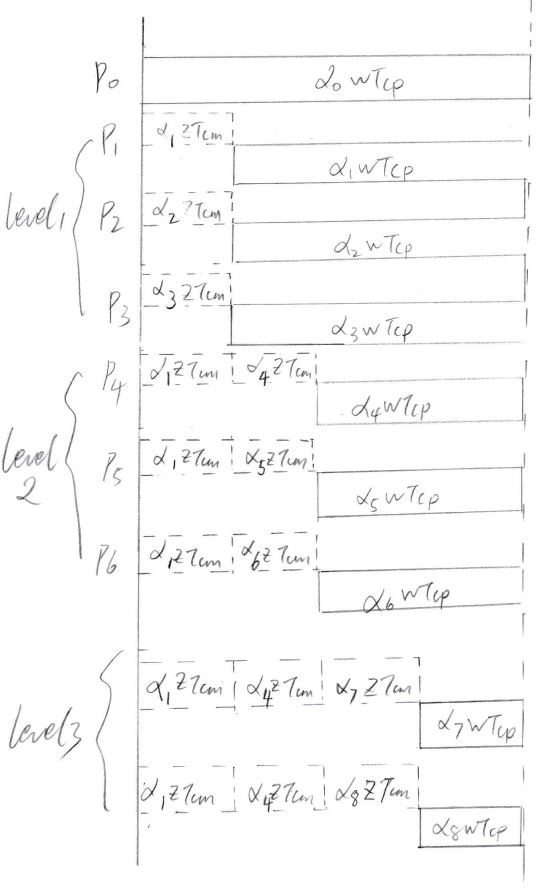
\includegraphics[width=0.5\columnwidth]{figure/3t3bd_no.JPG}
\caption{The timing diagram for 3*3 boundary data injection on $P_{0}$ }
\label{fig:3t3bd_no}
\end{figure}
The equations are:
\begin{empheq}[left=\empheqlbrace]
{align}
\alpha_{0} \omega T_{cp} = T_{f, m}\\
\alpha_{1}zT_{cm} + \alpha_{1} \omega T_{cp} = T_{f, m}\\
\alpha_{2}zT_{cm} + \alpha_{2} \omega T_{cp} = T_{f, m}\\
\alpha_{3}zT_{cm} + \alpha_{3} \omega T_{cp} = T_{f, m}\\
(\alpha_{1} + \alpha_{4})zT_{cm} + \alpha_{4}\omega T_{cp} = T_{f, m}\\
(\alpha_{2} + \alpha_{5})zT_{cm} + \alpha_{5}\omega T_{cp} = T_{f, m}\\
(\alpha_{3} + \alpha_{6})zT_{cm} + \alpha_{6}\omega T_{cp} = T_{f, m}\\
(\alpha_{1} + \alpha_{4} +\alpha_{7})zT_{cm} + \alpha_{7}\omega T_{cp} = T_{f, m}\\
(\alpha_{1} + \alpha_{4} +\alpha_{8})zT_{cm} + \alpha_{8}\omega T_{cp} = T_{f, m}\\
\sigma = \frac{zT_{cm}}{\omega T_{cp}}\\
0 < \sigma < 1 \\
0 < \alpha_{0} \leq 1\\
0 \leq \quad \alpha_{1} \quad \alpha_{3} \quad \alpha_{4} \quad \alpha_{5} \quad \alpha_{6} \quad \alpha_{7} \quad \alpha_{8}  < 1
\end{empheq}
The flow matrix is :
\begin{equation}
{
\left[ \begin{array}{cccc}
1 & 3 & 3 & 2\\
1 & -(\sigma + 1) & 0 & 0\\
1 & -\sigma & -(\sigma + 1) & 0\\
1 & -\sigma & -\sigma & -(\sigma + 1)
\end{array} 
\right ]} \times \left[ \begin{array}{c}
\alpha_{0} \\
\alpha_{1} \\
\alpha_{4} \\
\alpha_{7}
\end{array} 
\right ] = \left[ \begin{array}{c}
1 \\
0 \\
0 \\
0
\end{array} 
\right ]
\end{equation}
\newpage 
The simulation result is shown in :
\begin{figure}[!ht]
\centering
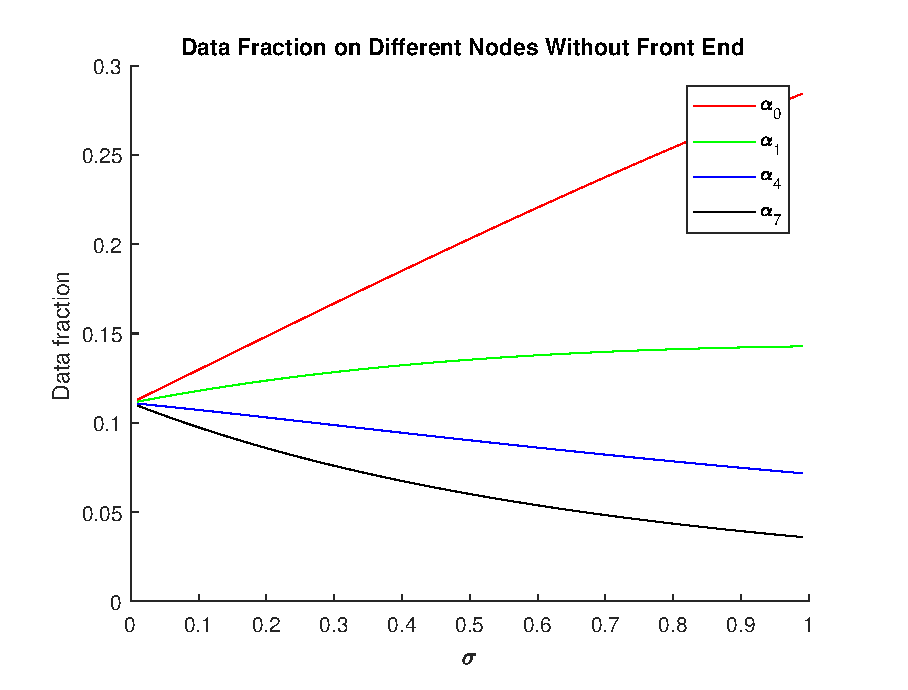
\includegraphics[width=1\columnwidth]{figure/3t3b_no_fraction.eps}
\caption{The fraction curve for 3*3 boundary data injection on $P_{0}$ }
\label{fig:3t3b_no_fraction}
\end{figure}

\newpage

\subsection{Data Injection on The Inner Grid Processor}
The equations are:
\begin{empheq}[left=\empheqlbrace]
{align}
\alpha_{0} \omega T_{cp} = T_{f, m}\\
\alpha_{1}zT_{cm} + \alpha_{1} \omega T_{cp} = T_{f, m}\\
\alpha_{2}zT_{cm} + \alpha_{2} \omega T_{cp} = T_{f, m}\\
\alpha_{3}zT_{cm} + \alpha_{3} \omega T_{cp} = T_{f, m}\\
\alpha_{4}zT_{cm} + \alpha_{4} \omega T_{cp} = T_{f, m}\\
(\alpha_{1} + \alpha_{5})zT_{cm} + \alpha_{5}\omega T_{cp} = T_{f, m}\\
(\alpha_{2} + \alpha_{6})zT_{cm} + \alpha_{6}\omega T_{cp} = T_{f, m}\\
(\alpha_{3} + \alpha_{7})zT_{cm} + \alpha_{7}\omega T_{cp} = T_{f, m}\\
(\alpha_{4} + \alpha_{8})zT_{cm} + \alpha_{8}\omega T_{cp} = T_{f, m}\\
\sigma = \frac{zT_{cm}}{\omega T_{cp}}\\
0 < \sigma < 1 \\
0 < \alpha_{0} \leq 1\\
0 \leq \quad \alpha_{1} \quad \alpha_{3} \quad \alpha_{4} \quad \alpha_{5} \quad \alpha_{6} \quad \alpha_{7} \quad \alpha_{8}  < 1
\end{empheq}
The flow matrix closed-form is:
\begin{equation}
{
\left[ \begin{array}{ccc}
1 & 4 & 4 \\
1 & -(\sigma + 1) & 0\\
1 & -\sigma & -(\sigma + 1)\\
\end{array} 
\right ]} \times \left[ \begin{array}{c}
\alpha_{0} \\
\alpha_{1} \\
\alpha_{5} \\
\end{array} 
\right ] = \left[ \begin{array}{c}
1 \\
0 \\
0 
\end{array} 
\right ]
\end{equation}

The simulation result shows:
\begin{figure}[!ht]
\centering
\includegraphics[width=1\columnwidth]{figure/4t4i_no_fraction.eps}
\caption{The timing diagram for 3*3 inner grid injection $P_{0}$ }
\label{fig:4t4i_no_fraction}
\end{figure}
\newpage